\documentclass{standalone}
\standaloneconfig{border=2mm 2mm 2mm 2mm}
%Packages & Librariesresultant-vector
\usepackage{tikz}
\usepackage{gensymb}
\usepackage{textcomp}
\usetikzlibrary{calc}

\begin{document}

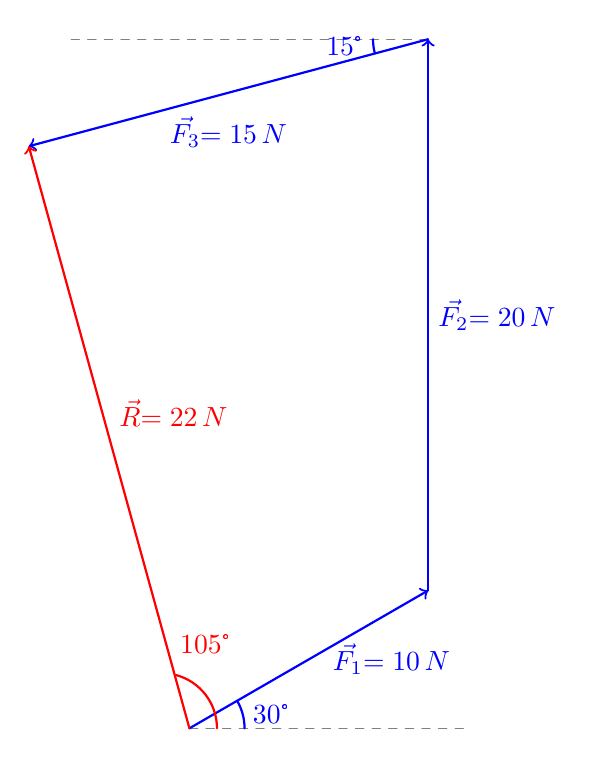
\begin{tikzpicture}[line cap=round,scale=0.35]
% Axes
\draw[dashed,gray] (0,0) -- (10,0); %x     
% Define the origin
\coordinate (O) at (0,0);    
% Define velocities v1, v2 and v3
\coordinate (A) at (8.66025,5); % Vector v1
\coordinate (B) at (0,20); % Vector v2
\coordinate (C) at (-14.4889,-3.8823); % Vector v3

% Draw vector v1
\draw[->, thick, blue] (O) -- (A) node[midway, right=5pt] {$\vec{F_1}{=10\,N}$};
\draw[thick, blue] (2,0) arc (0:30:2) node[midway, right]{$30\degree$};   
% Draw vector v2 starting from the tip of v1
\draw[->, thick, blue] (A) -- ($(A)+(B)$) node[midway, right] {$\vec{F_2}{=20\, N}$} coordinate (B');   
\draw[dashed,gray] (B') -- ++(-13,0); % Relative and Incremental Coordinates   
\draw[thick, blue] ($(B')+(-2,0)$) arc (180:195:2) node[midway, left]{$15\degree$};
% Draw vector v3 starting from the tip of v2
\draw[->, thick, blue] (B') -- ($(B')+(C)$) node[midway, below=5pt] {$\vec{F_3}{=15\, N}$} coordinate (C');
% Draw the resulting vector from the origin to the end of v3
\draw[red, ->, thick] (O) -- (C') node[midway, above right] {$\vec{R}{=22\, N}$};
\draw[thick, red] (1,0) arc (0:75:2) node[midway, above=11pt]{$105\degree$};
\end{tikzpicture}

\end{document}